\clearpage
\section{improved TEP-Net}

blindtext

\subsection{Backbones}

\begin{table}[H]
    \centering
    \resizebox{\textwidth}{!}{
        \begin{tabular}{lcccccc}
            \hline
            \rowcolor{white} \textbf{Model} & \textbf{Parameters} & \textbf{Flops} & \textbf{MACs} & \textbf{Latency TRT FP32 / FP16} & \textbf{IoU} & \textbf{Switch Eval} \\
            \hline
            \rowcolor[gray]{0.9} ENB3 \cite{tepNet2024} & 14.57M & 9.74B          & 5.16G          & 24.89 / 15.26 ms        & \textbf{97.53 \%} & 91.18 \% \\ 
            \rowcolor{white}     RN18 \cite{tepNet2024} & 15.64M & 18.98B         & 9.53G          & 9.48 / 3.25 ms          & 96.95 \%          & 80.15 \% \\ 
            \hline
            \rowcolor[gray]{0.9} MNV3-Small & \textbf{5.33M}     & \textbf{0.55B} & \textbf{0.30G} & \textbf{3.13 / 2.05 ms} & 96.19 \%          & 73.53 \% \\ 
            \rowcolor{white}     MNV3-Large & 7.27M              & 2.15B          & 1.17G          & 6.41 / 3.75 ms          & 96.49 \%          &  \\ 
            \rowcolor[gray]{0.9} DN121      & 11.42M             & 29.61B         & 15.14G         & 29.53 / 16.52 ms        & 97.50 \%          &  \\ 
            \rowcolor{white}     DN161      & 30.9M              & 80.74B         & 40.98G         & 75.77 / 34.02 ms        & 97.46 \%          &  \\ 
            \rowcolor[gray]{0.9} DN169      & 16.96M             & 35.10B         & 17.95G         & 38.87 / 22.51 ms        & 97.48 \%          &  \\ 
            \rowcolor{white}     DN201      & 22.57M             & 44.83B         & 22.93G         & 52.14 / 29.94 ms        & 97.51 \%          & \textbf{93.38 \%}  \\
            \hline
        \end{tabular}
    }
    \caption{Backbone Results}
    \label{tab:backboneResults}
\end{table}

\autoref{tab:backboneResults} shows the results of models with different backbones.
Since \cite{tepNet2024} already implemented various versions of ResNet and EfficientNet.
Their results showed that ResNet18 is the fastest model and EfficientNet-B3 is the most accurate according to the \ac{IoU}.
\autoref{tab:backboneResults} shows these results for a better overview and comparison.
Data for those two models is from \cite{tepNet2024}, which does not give information about Flops.
Nevertheless, those two models are evaluated on the switch evaluation dataset for performance comparison considering switch cases.
All versions of MobileNetV3 and DenseNet available on PyTorch are implemented and evaluated.
Only the most accurate DenseNet version according to the \ac{IoU} and the fastest model, the MoblieNetV3-Small, are assessed on the switch evaluation dataset.

\autoref{tab:backboneResults} shows an apparent gain in speed with the MobleNetV3s and the Small version being the fastest with latencies of only 2.05 ms on the Jetson AGX Xavier when quantized to FP16 with TensorRT.
This duration is equivalent to 487.8 \ac{FPS}.
Compared to EfficientNetB3, this is 7.44 times faster while only losing 1.34\% of the \ac{IoU} accuracy.
The MobielNetV3-Small is the most lightweight model with only 5.33M Parameters.
However, this backbone shows more confusion when considering switch cases because performance drops significantly on the switch evaluation dataset.

The DenseNet201 outperformed all other models on the switch evaluation dataset with correct predictions of 93.38\%.
However, latency increases remarkably with durations of 52.14 ms for FP32 and 29.94 ms for FP16.
Equivalent to 19.17 \ac{FPS} and 33.4 \ac{FPS}, respectively, the FP32 quantized model would not be real-time capable when inferring 30 \ac{FPS} videos.
Since the FP16 model also closely approaches the boundary, DenseNets are excluded from further investigations.

\autoref{tab:backboneResults} shows the best values in each category in bold.
Since these values spread across various models, further experiments must be conducted to determine a final backbone.
Until now, only DenseNets are excluded.

\subsection{Pooling Layers}

\begin{table}[H]
    \centering
    \hspace{-3cm}
    \begin{minipage}{0.03\textwidth} % Für den vertikal gedrehten Text
        \rotatebox{90}{\textbf{\hspace{0.5cm} Max Pool \hspace{0.5cm} Average Pool \hspace{0.8cm} No Pool \hspace{1cm}}}
    \end{minipage}%
    \resizebox{0.95\textwidth}{!}{
    \begin{minipage}{0.95\textwidth} % Für die Tabelle
        \begin{tabular}{lcccccc}
            \hline
            \rowcolor{white} \textbf{Model} & \textbf{Parameters} & \textbf{Flops} & \textbf{MACs} & \textbf{Latency TRT FP32 / FP16} & \textbf{IoU} & \textbf{Switch Eval} \\
            \hline
            \rowcolor[gray]{0.9} ENB3 \cite{tepNet2024} & 14.57M   & 9.74B          & 5.16G          & 24.89 / 15.26 ms        & \textbf{97.53 \%} & 91.18 \% \\ 
            \rowcolor{white}     RN18 \cite{tepNet2024} & 15.64M   & 18.98B         & 9.53G          & 9.48 / 3.25 ms          & 96.95 \%          & 80.15 \% \\ 
            \rowcolor[gray]{0.9} MNV3-Small    & \textbf{5.33M}    & \textbf{0.55B} & \textbf{0.30G} & \textbf{3.13 / 2.05 ms} & 96.19 \%          & 73.53 \% \\ 
            \rowcolor{white}     DN201         & 22.57M            & 44.83B         & 22.93G         & 52.14 / 29.94 ms        & 97.51 \%          & 93.38 \% \\
            \hline
            \rowcolor[gray]{0.9} ENB3-AP       & 15.35M            & 10.13B         & 5.36G          & 25.64 / 15.25 ms        & 91.34 \%          & 93.38 \% \\ 
            \rowcolor{white}     RN18-AP       & 16.69M            & 19.49B         & 9.8G           & 10.18 / 3.42 ms         & 96.58 \%          & 91.18 \% \\ 
            \rowcolor[gray]{0.9} MNV3-Small-AP & 5.53M             & 0.65B          & 0.35G          & 3.24 / 2.1 ms           & 95.02 \%          & 58.82 \% \\ 
            \rowcolor{white}     DN201-AP      & -                 & -              & -              & Expected to be high     & -                 & - \\ 
            \hline
            \rowcolor[gray]{0.9} ENB3-MP       & 15.35M            & 10.13B         & 5.36G          & 25.68 / 15.5 ms         & 97.30 \%          & \textbf{94.85} \% \\ 
            \rowcolor{white}     RN18-MP       & 16.69M            & 19.49B         & 9.8G           & 9.89 / 3.41 ms          & 96.88 \%          & 91.91 \% \\ 
            \rowcolor[gray]{0.9} MNV3-Small-MP & 5.53M             & 0.65B          & 0.35G          & 3.25 / 2.11 ms          & 95.95 \%          & 68.38 \% \\ 
            \rowcolor{white}     DN201-MP      & -                 & -              & -              & Expected to be high     & -                 & - \\ 
            \hline
        \end{tabular}
    \end{minipage}
    }
    \caption{Pooling Layers Results}
    \label{tab:poolongResults}
\end{table}

Further improvements are the added actual pooling layers after the backbone.
For this, models with EfficientNetB3, ResNet18, and MobileNetV3-Small are evaluated.
These models, including DenseNet201, are shown in the first four rows of \autoref{tab:poolongResults} with no pooling to visualize the differences in performance better.

An adaptive average or max pool is implemented for pooling layers.
This work evaluates the three models with both layers.
\autoref{tab:poolongResults} shows that the performance of the MobileNet according to the switch evaluation dataset drops even further with both pooling layers.
Since this work predominantly focuses on switch cases and the direction of the train is more critical than pixel-level accuracy, MobileNets are not further considered in this work.

The best trade-off between accuracy and speed provides the EfficientNetB3 with an integrated max pooling layer.
It outperforms others according to the switch accuracy with 94.85\%.
Additionally, the \ac{IoU} shows great pixel-level accuracy.
It is only 0.23\% less accurate than the best-performing model in this category, which has the same backbone but without a pooling layer.
Its latencies of 25.68 ms for FP32 and 15.5 ms for FP16 correspond to speeds up to 38.94 \ac{FPS} and 64.51 \ac{FPS}, which leaves a sufficiently large margin for additional enhancements.
Therefore, the ENB3-MP is selected for further investigation with various prediction heads.

\subsection{Prediction Heads}

\begin{table}[H]
    \centering
    \resizebox{\textwidth}{!}{
    \begin{tabular}{lcccccc}
        \hline
        \rowcolor{white} \textbf{Model} & \textbf{Parameters} & \textbf{Flops} & \textbf{MACs} & \textbf{Latency TRT FP32 / FP16} & \textbf{IoU} & \textbf{Switch Eval} \\
        \hline
        \rowcolor[gray]{0.9} ENB3-MP      & \textbf{15.35M} & \textbf{10.13B} & \textbf{5.36G} & \textbf{25.68 / 15.5 ms}  & \textbf{0.9730} & 94.85 \% \\ 
        \hline
        \rowcolor{white}     DEPTH-HEAD   & 23.75M & 10.15B & 5.37G & 25.57 / 15.74 ms & 0.9721 & 91.91 \% \\ 
        \rowcolor[gray]{0.9} WIDTH-HEAD   & 36.59M & 10.18B & 5.38G & 26.51 / 16.09 ms & 0.9723 & 97.06 \% \\ 
        \rowcolor{white}     TRAPEZE-HEAD & 32.92M & 10.17B & 5.38G & 25.87 / 16.09 ms & 0.9715 & \textbf{97.79} \% \\ 
        \hline
    \end{tabular}
    }
    \caption{Prediction Heads Results}
    \label{tab:predHeadsResults}
\end{table}

The model with the EfficientNetB3 backbone and an included adaptive max pooling layer outperformed others.
Therefore, this model is equipped with different prediction heads for further investigation.
\autoref{subsubsec:predictionheads} describes the various heads in detail.
They all show only a slight increase in latency.
However, according to the evaluation on switches, the best-performing model is the model with the trapeze head.
It achieves a switch accuracy of 97.79\% while only increasing the latency by 0.19 ms for FP32 and 0.59 ms for FP16.
Converted to \ac{FPS}, this corresponds to 38.65 and 62.15, respectively.
Since this latency gain is acceptable for almost an additional 3\% switch accuracy presents a good trade-off, the final model incorporates the EfficientNet-B3 backbone, an adaptive max pooling layer, and the introduced trapeze head.

\section{Qualitative comparison between the baseline model and the improved Version}

\begin{figure}[H]
    \centering
    \begin{minipage}{0.2\textwidth} % Linke Seite für Text
        \centering
        \textbf{original TEP-Net}\\
        EfficientNet-B3
    \end{minipage}%
    \hfill
    \begin{minipage}{0.6\textwidth} % Mittlere Spalte für die Figure
        \centering
        % Hier die Original-Figur
        \begin{subfigure}[b]{0.48\textwidth}
            \centering
            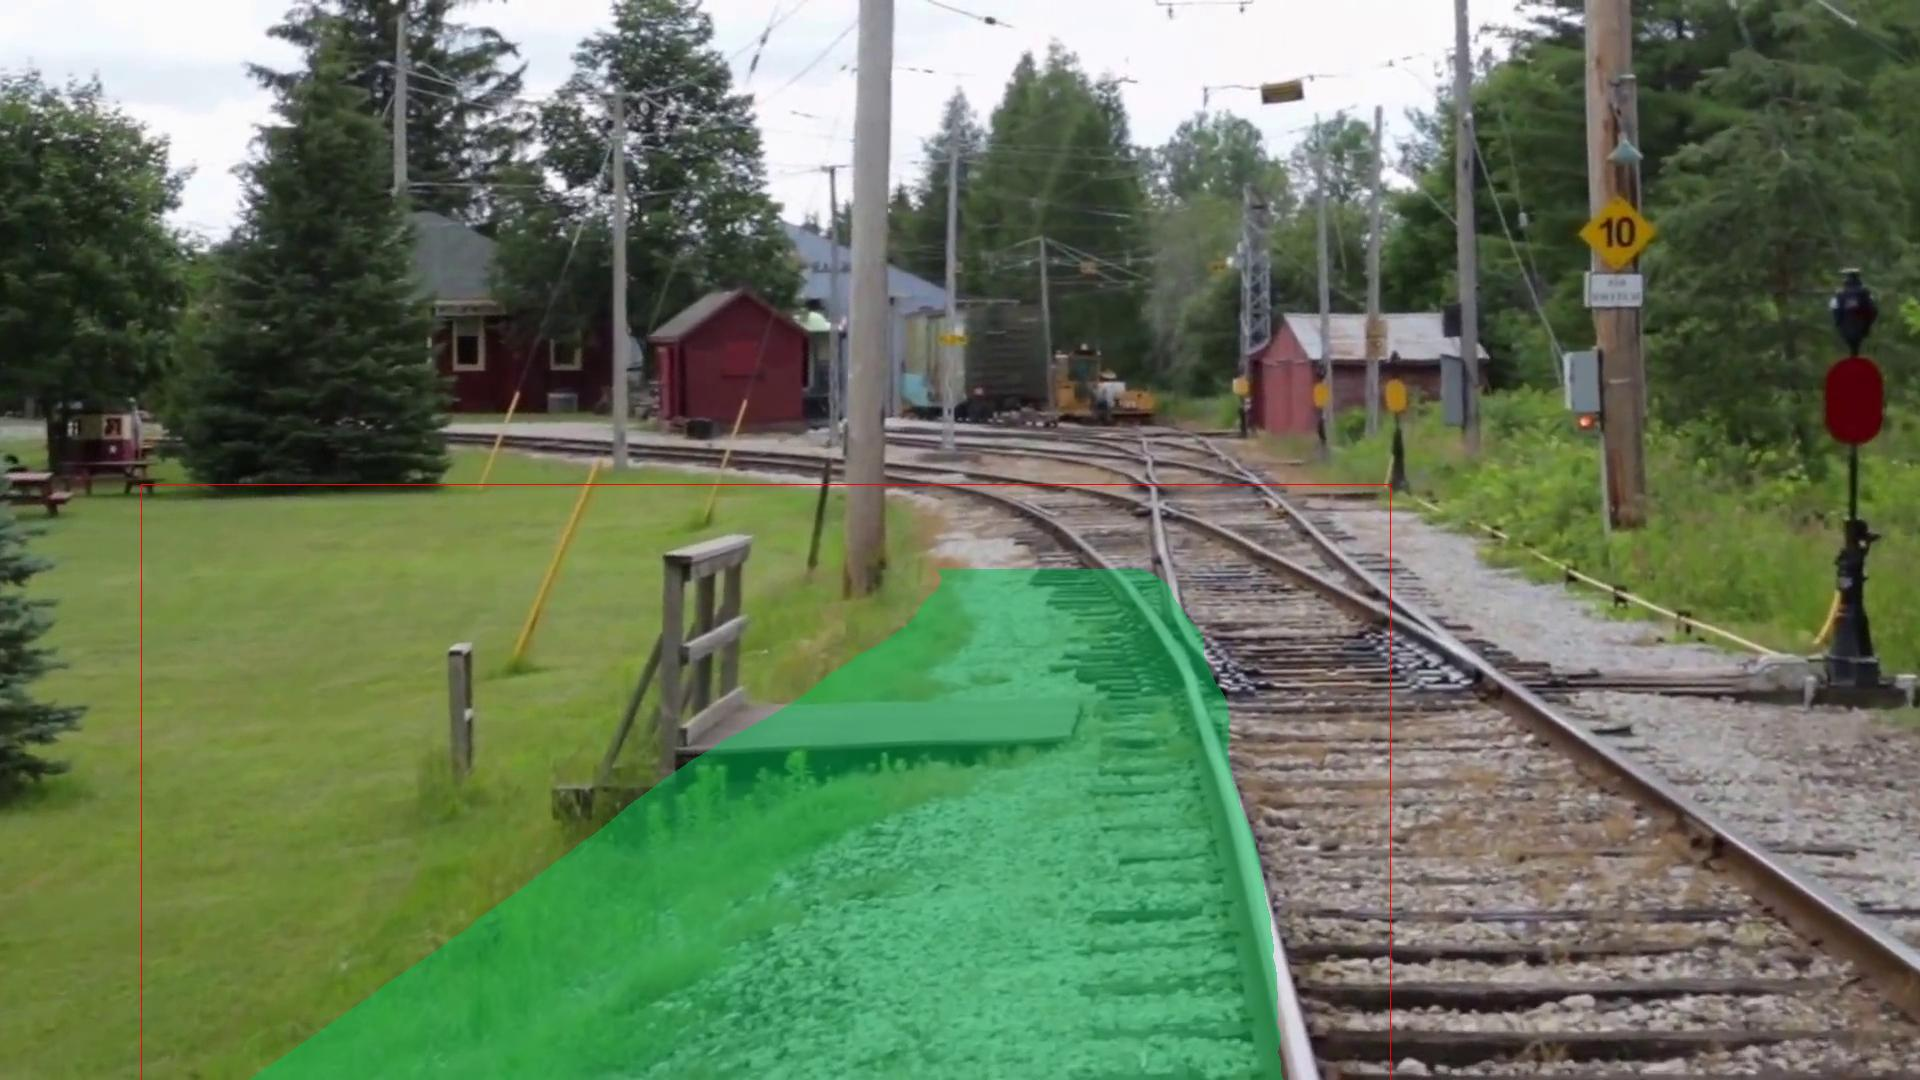
\includegraphics[width=\textwidth]{PICs/experiments/ComparisonBaselineToImproved/original2.jpg}
        \end{subfigure}
        \begin{subfigure}[b]{0.48\textwidth}
            \centering
            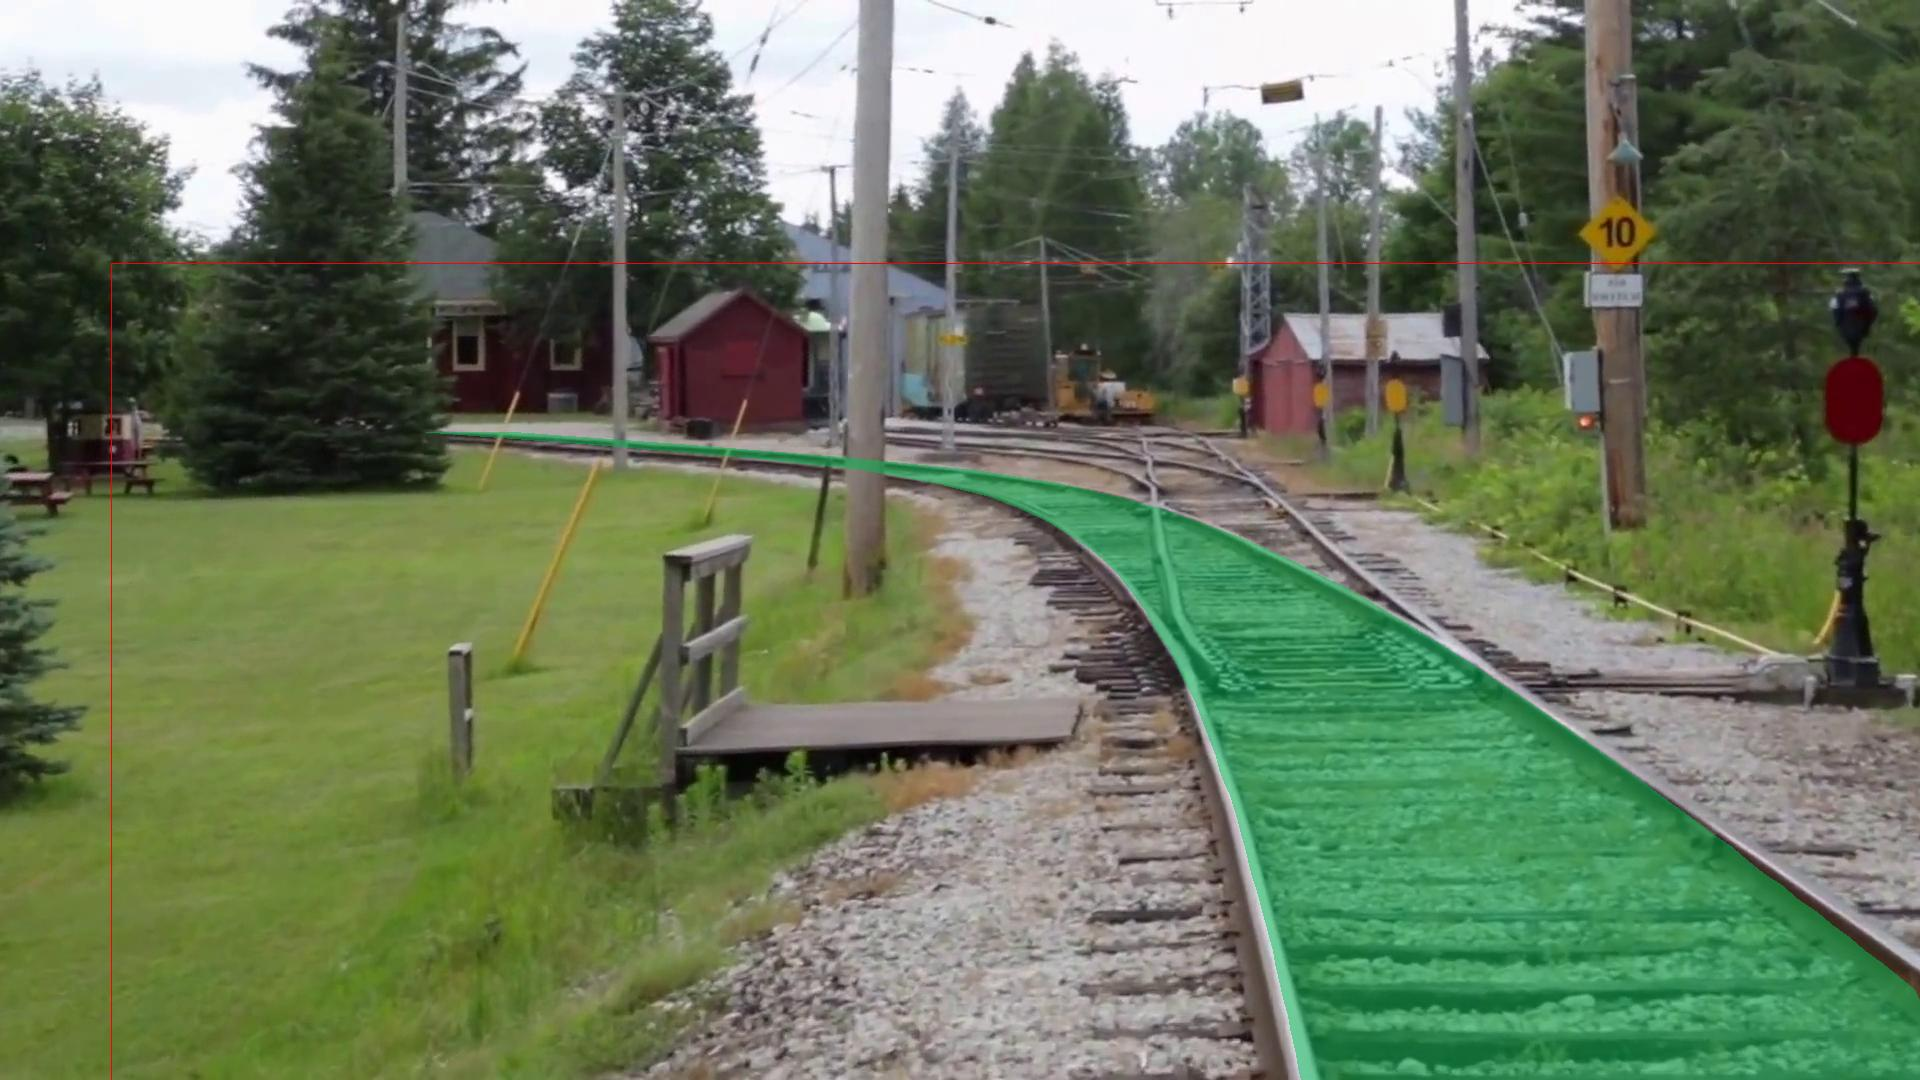
\includegraphics[width=\textwidth]{PICs/experiments/ComparisonBaselineToImproved/adapted2.jpg}
        \end{subfigure}
        
        \vspace{0.5cm} % Abstand zwischen den Zeilen
        
        \begin{subfigure}[b]{0.48\textwidth}
            \centering
            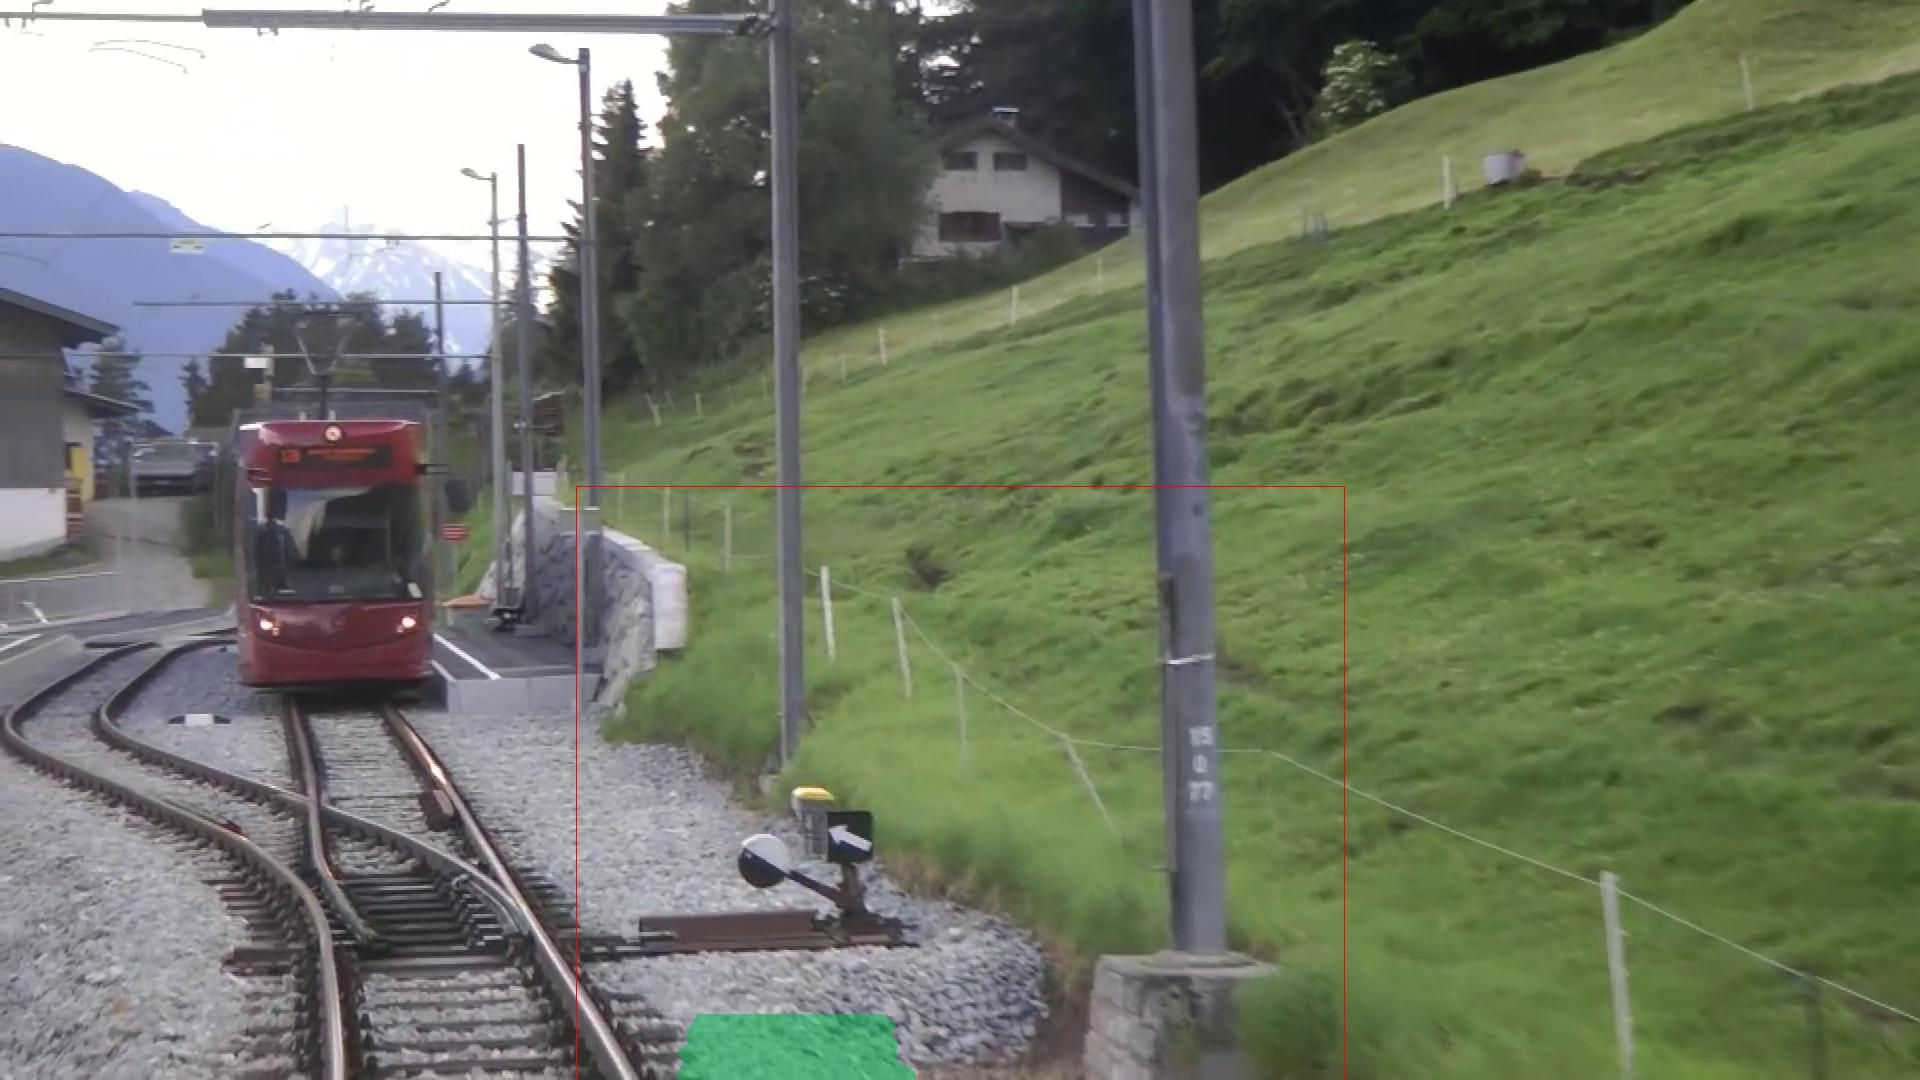
\includegraphics[width=\textwidth]{PICs/experiments/ComparisonBaselineToImproved/original1.jpg}
        \end{subfigure}
        \begin{subfigure}[b]{0.48\textwidth}
            \centering
            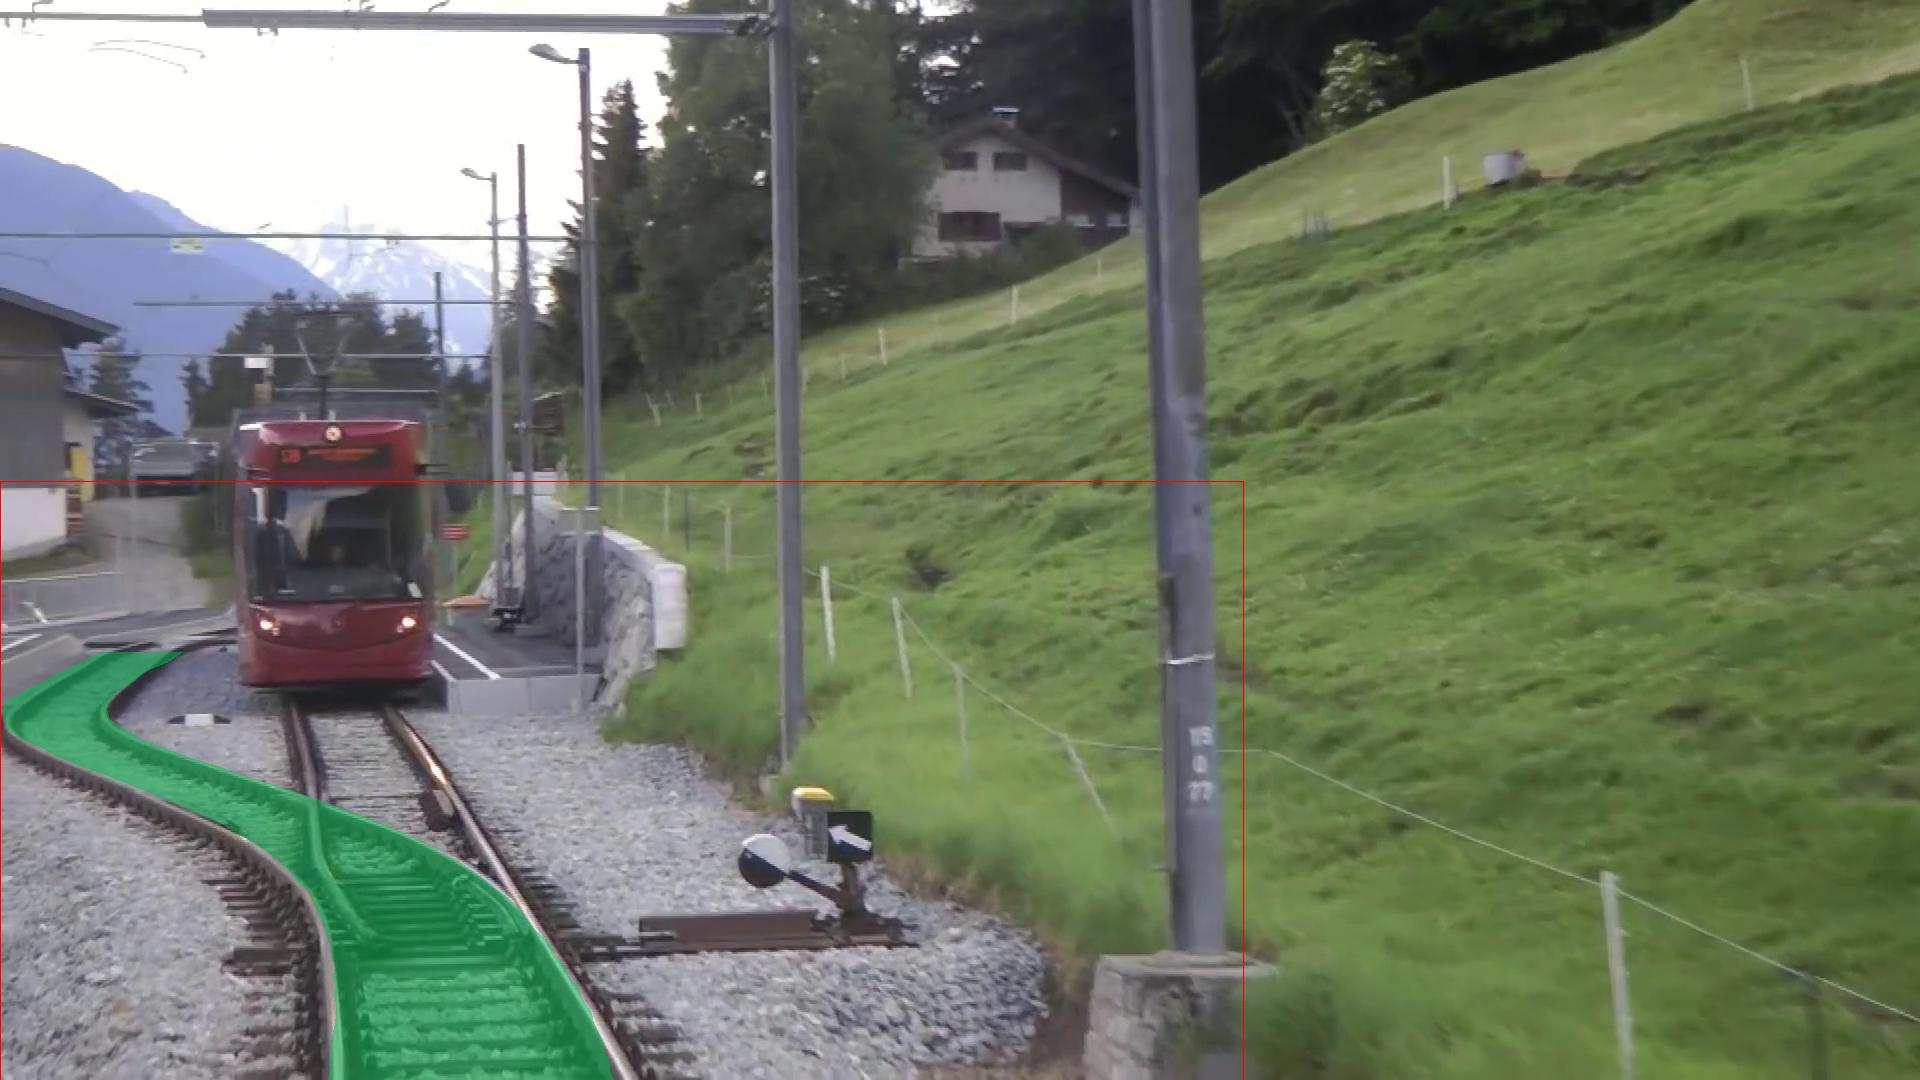
\includegraphics[width=\textwidth]{PICs/experiments/ComparisonBaselineToImproved/adapted1.jpg}
        \end{subfigure}
        
        \vspace{0.5cm} % Abstand zwischen den Zeilen
        
        \begin{subfigure}[b]{0.48\textwidth}
            \centering
            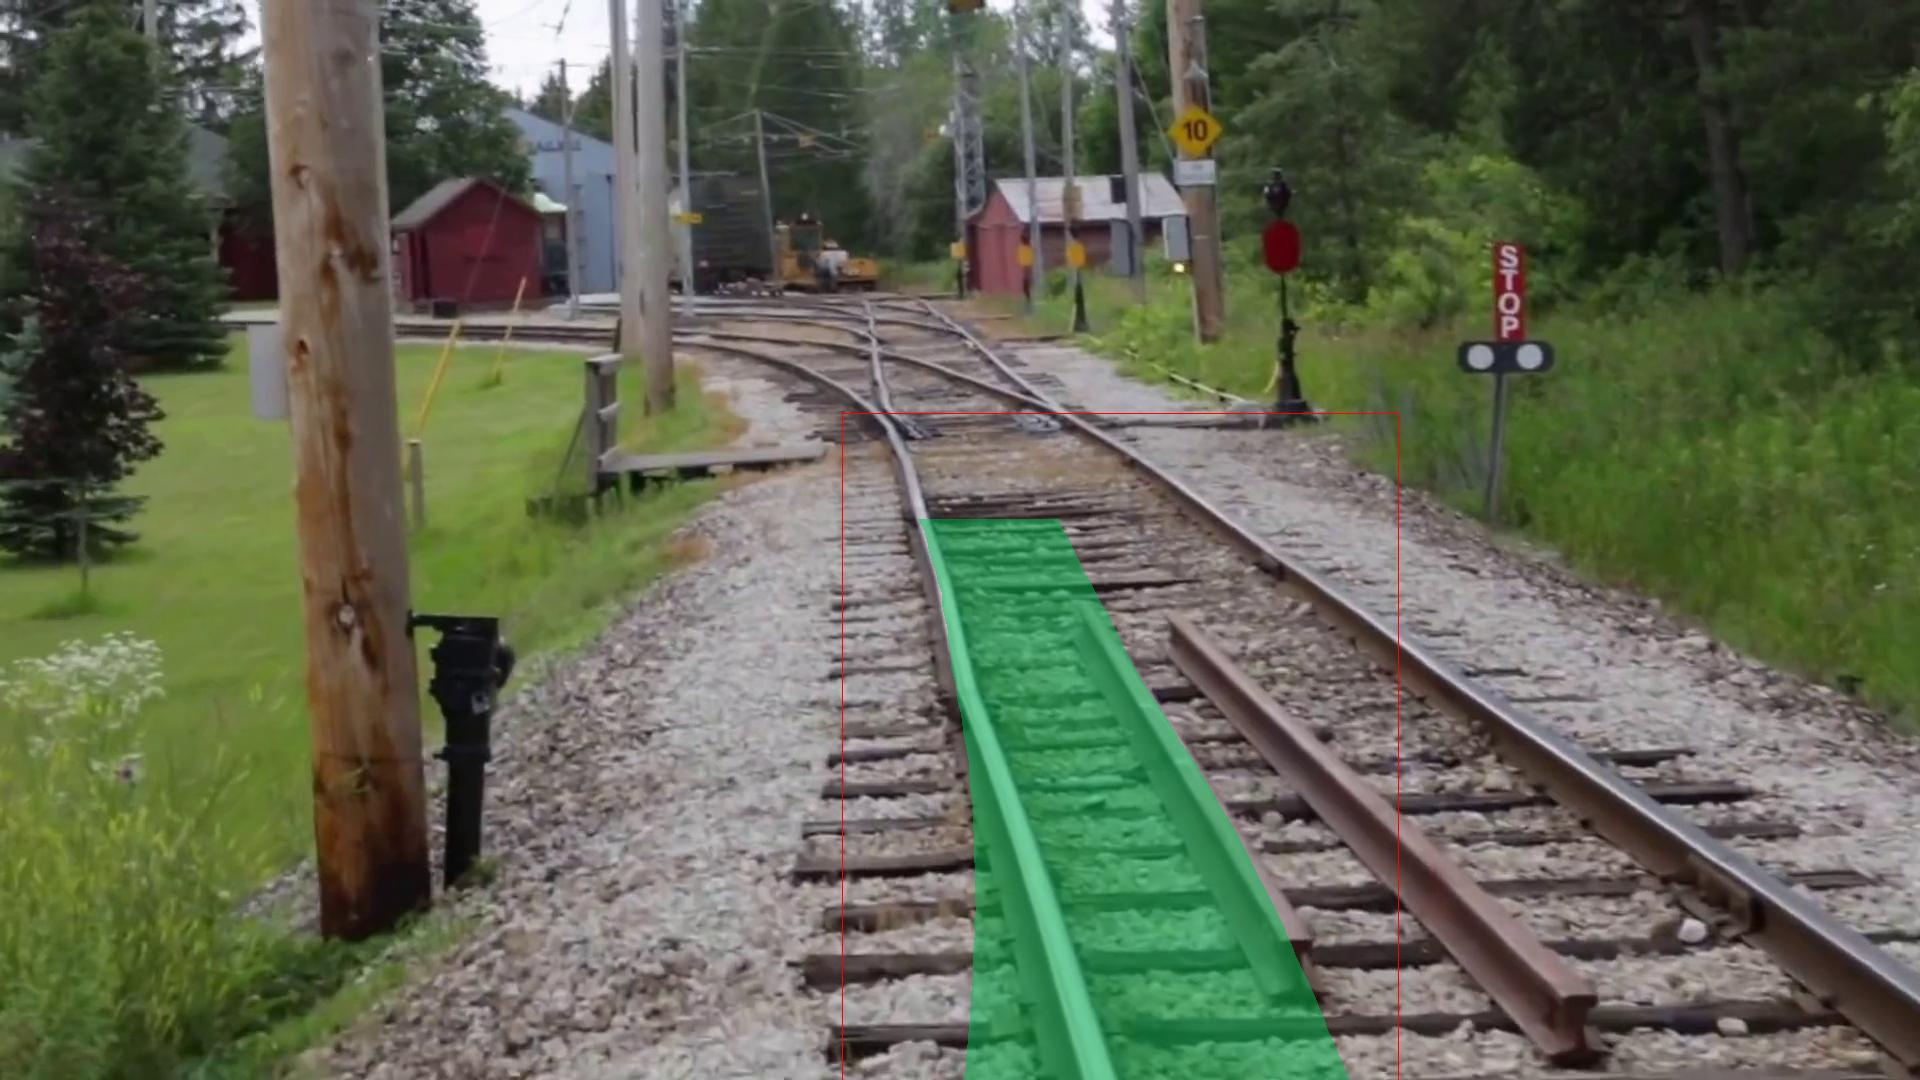
\includegraphics[width=\textwidth]{PICs/experiments/ComparisonBaselineToImproved/original3.jpg}
        \end{subfigure}
        \begin{subfigure}[b]{0.48\textwidth}
            \centering
            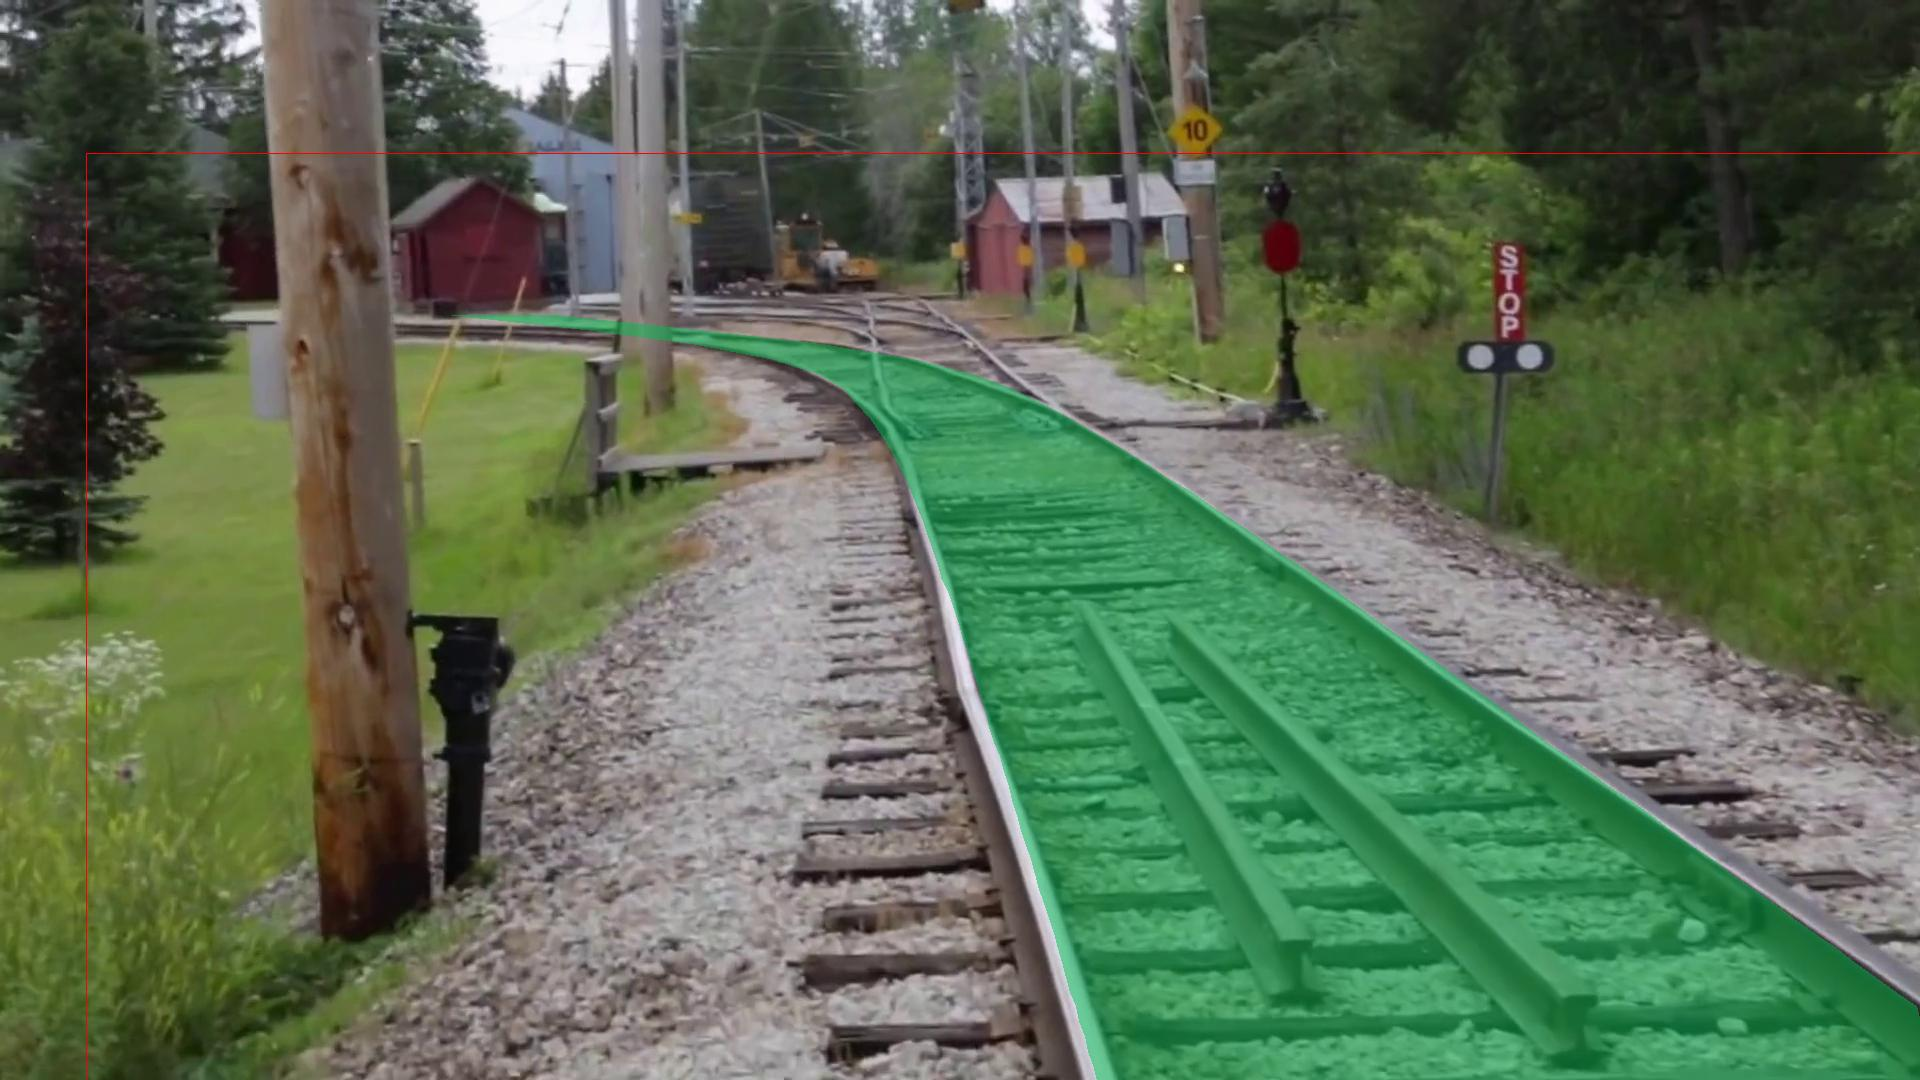
\includegraphics[width=\textwidth]{PICs/experiments/ComparisonBaselineToImproved/adapted3.jpg}
        \end{subfigure}
    \end{minipage}%
    \hfill
    \begin{minipage}{0.2\textwidth} % Rechte Seite für Text
        \centering
        \textbf{adapted TEP-Net}\\
        EfficientNet-B3
    \end{minipage}
    \caption{Comparison between the best version of TEP-Net \cite{tepNet2024} and the best version with all improvements of this work: best backbone, adaptive max pooling, trapeze head and adapted auto-crop mechanism.
    Images of complex scenes with difficult angles of perspective are intenionally chosen.}
    \label{fig:comparisonBaseline2Improved}
\end{figure}

\autoref{fig:comparisonBaseline2Improved} shows three examples of the switch evaluation dataset.
These predictions are obtained with the auto-cropping mechanism.
The crop coordinates are adjusted by predicting each image 50 times.
On the left, predictions are made with the best-performing model from \cite{tepNet2024} with the original auto cropping technique, and on the right, all introduced improvements are used.
That includes the adapted auto crop mechanism and best-performing model incorporating an EfficientNet-B3 backbone, the adaptive max pooling layer, and the trapeze head.

For this brief qualitative comparison, three images with intentionally complex scenes are chosen to view differences more clearly.
That includes rails captured from very unusual angles that do not start from the bottom center like most other images from the dataset.
In the image in the bottom row, additional rails lay in the track, introducing an extra challenge.

\autoref{fig:comparisonBaseline2Improved} visualizes that the original model \cite{tepNet2024} struggles to find the track.
The improved Version finds the track and correctly predicts the switch in each image, which proves that all introduced adaptations increase the system's robustness and thus enhance safety in a practical application.
